\chapter{Photogrammetrie}

\section{Einführung in die Photogrammetrie}

Das Grundprinzip der Messung mit Kameras ist einfach. Licht breitet sich mit einer bestimmten Wellenlänge, in annähernd geraden Strahlen aus. Diese Strahlen werden vom Sensor der Kamera aufgenommen, sodass diese die Richtungen im dreidimensionalen Raum misst. Der grundlegende geometrische Zusammenhang der Photogrammetrie ist somit die Zentralprojektion, die sich mathematisch durch die Kollinearitätsgleichung beschreiben lässt. Ein dreidimensionaler Punkt in der echten Welt, sein Bild in der Kamera und das Projektionszentrum müssen alle auf einer geraden Linie liegen. (vgl. \cite{fiundations_pg} S.1) Das fundamentale photogrammetrische Problem besteht in der Bestimmung von internen und externen Ausrichtungsparametern der Kamera und der  Messung von Objekt und Raumkoordinaten der aufgenommenen Fotografien. 


\begin{itemize}
\item \textbf{Interne Orientierung}: Bei der internen Orientierung werden Kameraparameter gemessen und ausgewertet. Dazu wird die \glqq principle distance\grqq{} (Brennweite) und der \glqq principle point\grqq{} (Optisches Zentrum) betrachtet.

\begin{figure}[H]
	\centering
	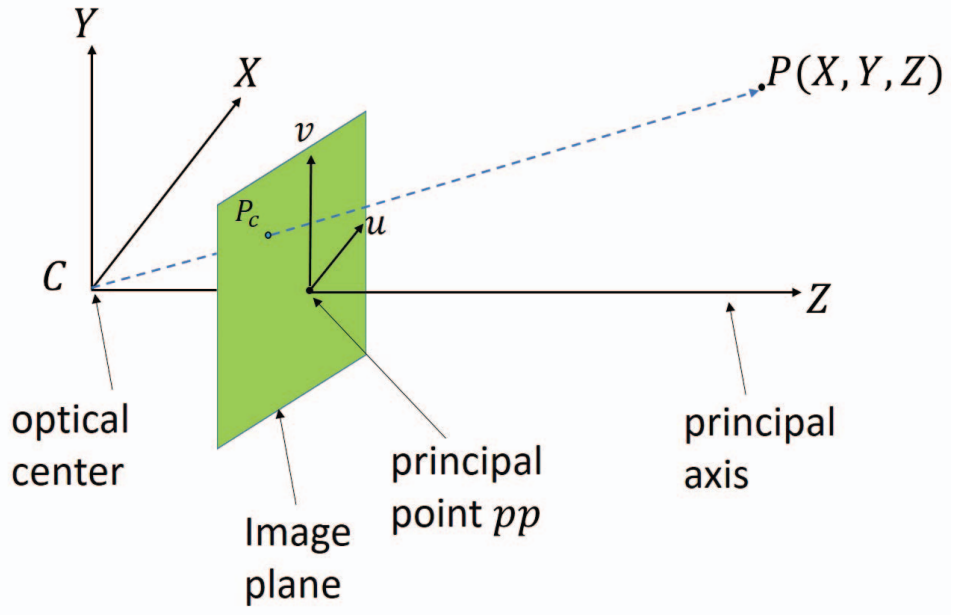
\includegraphics[scale=0.45]{pp.png}
	\caption{Kamera Kalibierungsmodell, Bildquelle \cite{pp}}
\end{figure} 

Weiterhin müssen Parameter, welche die Verzeichnung, also die nicht maßstabsgetreue Abbildung von Objekten, betrachtet werden. Diese Parameter, die beispielsweise in der Objektivkorrektur verwendet werden, müssen, um die interne Orientierung der Kamera genau abzubilden, mit in die Berechnung einfließen.

\item \textbf{Externe Orientierung}: Bei der externen Orientierung wird versucht die genaue räumliche dreidimensionale Lage der Kamera zum Zeitpunkt der Belichtung des Bildes zu rekonstruieren. Für die Bestimmung der Orientierung von ein oder mehreren Fotos, können verschiedene Methoden verwendet werden. Dies kann in Teilschritten (relative und absolute Orientierung) oder gleichzeitig (Bündelblockausgleich) durchgeführt werden. (vgl. \cite{exterior_review} S.616)
\end{itemize}

Khalid El-AShmawy \cite{comparative_conditions_study} beschreibt die Verwendung von Strahlenbündel, die durch Fotos generiert werden, als zweifelsfrei den flexibelsten Ansatz zur Blockbildung, Blockanpassung und für Photogrammetrie im Allgemeinen und mit den besten Ergebnissen. In der Nahbereichsphotogrammetrie, bei der mehrstufige und konvergente Konfigurationen möglich sind, ist der Bündelansatz in seiner stärksten Form vertreten. 


Der Ausgleich der Strahlenbündel in einem Set an Fotos beinhaltet die Rotation und Translation von jedem Bündel im Raum in eine Position, in der alle Strahlen sich an der korrekten Position im Objektraum schneiden. (vgl. \cite{comparative_conditions_study} S.66)

\section{Bündelblockausgleich}

Das Verfahren des Bündelblockausgeleichs, verwendet die Methoden der \glqq collinearity condition \grqq{} (Kollinearitätsbedingung), der \glqq coplanarity condition\grqq{} (Koplanaritätsbedingung) oder die Methode der direkten linearen Transoformation. Die gewünschten Parameter aller Fotos werden gleichzeitig durch eine iterative Wiederholung der \glqq least square\grqq{} Methode (Methode der kleinsten Quadrate) angepasst und korrigiert. Die Iterationen sind durch die nicht-Linearität der Konditionsgleichungen notwendig. Die Resulate des Bündelblockausgleichs aller Fotos sind dann die Ergebnisse der externen Orientierung der Kamera für jedes einzelne Foto. Weiterhin ergibt sich eine Auflistung der Objektraumkoordinaten der gemessenen Punkte aller Fotos, sowie deren gemessene statische Genauigkeit. (vgl. \cite{comparative_conditions_study} S.66-67)

\url{https://ethz.ch/content/dam/ethz/special-interest/baug/igp/photogrammetry-remote-sensing-dam/documents/pdf/math-of-photogrammetry.pdf}
\url{http://sci-hub.tw/https://doi.org/10.3846/20296991.2015.1051335}
\url{http://sci-hub.tw/10.1111/0031-868X.00210}

\subsection{collinearity}

\subsection{coplanarity}

\subsection{direct linear transformation}

\subsection{Feature Matching}

\subsection{Image Matching}

\subsection{Structure from Motion}

6.2 Structure from motion

\url{http://sci-hub.tw/https://doi.org/10.1007/s10462-012-9365-8}

\subsection{Depth Maps}

\section{Photogrammetrie für Smartphones}

\section{Evaluierung der photogrammetrischen Technologie für Echtzeit AR Anwendungen}